\chapter*{Appendix B: metadata visualizations}\label{layer}

The physical parameter space of a set of BNS simulations can be represented using a layered plot, which stacks different physical observables for each simulation ID. Reading through simulation metadata using such a plot is much easier than dealing with data extraction and unit conversion, in case the developer of the catalog or simulations provides it. 

The following is a layered plot representing the total mass, mass ratio, tidal deformability, maximum TOV mass, and the effective spin parameter for the CoRe BNS catalog \cite{Dietrich:2018phi}.



\begin{figure}[hbt!]
\begin{center}
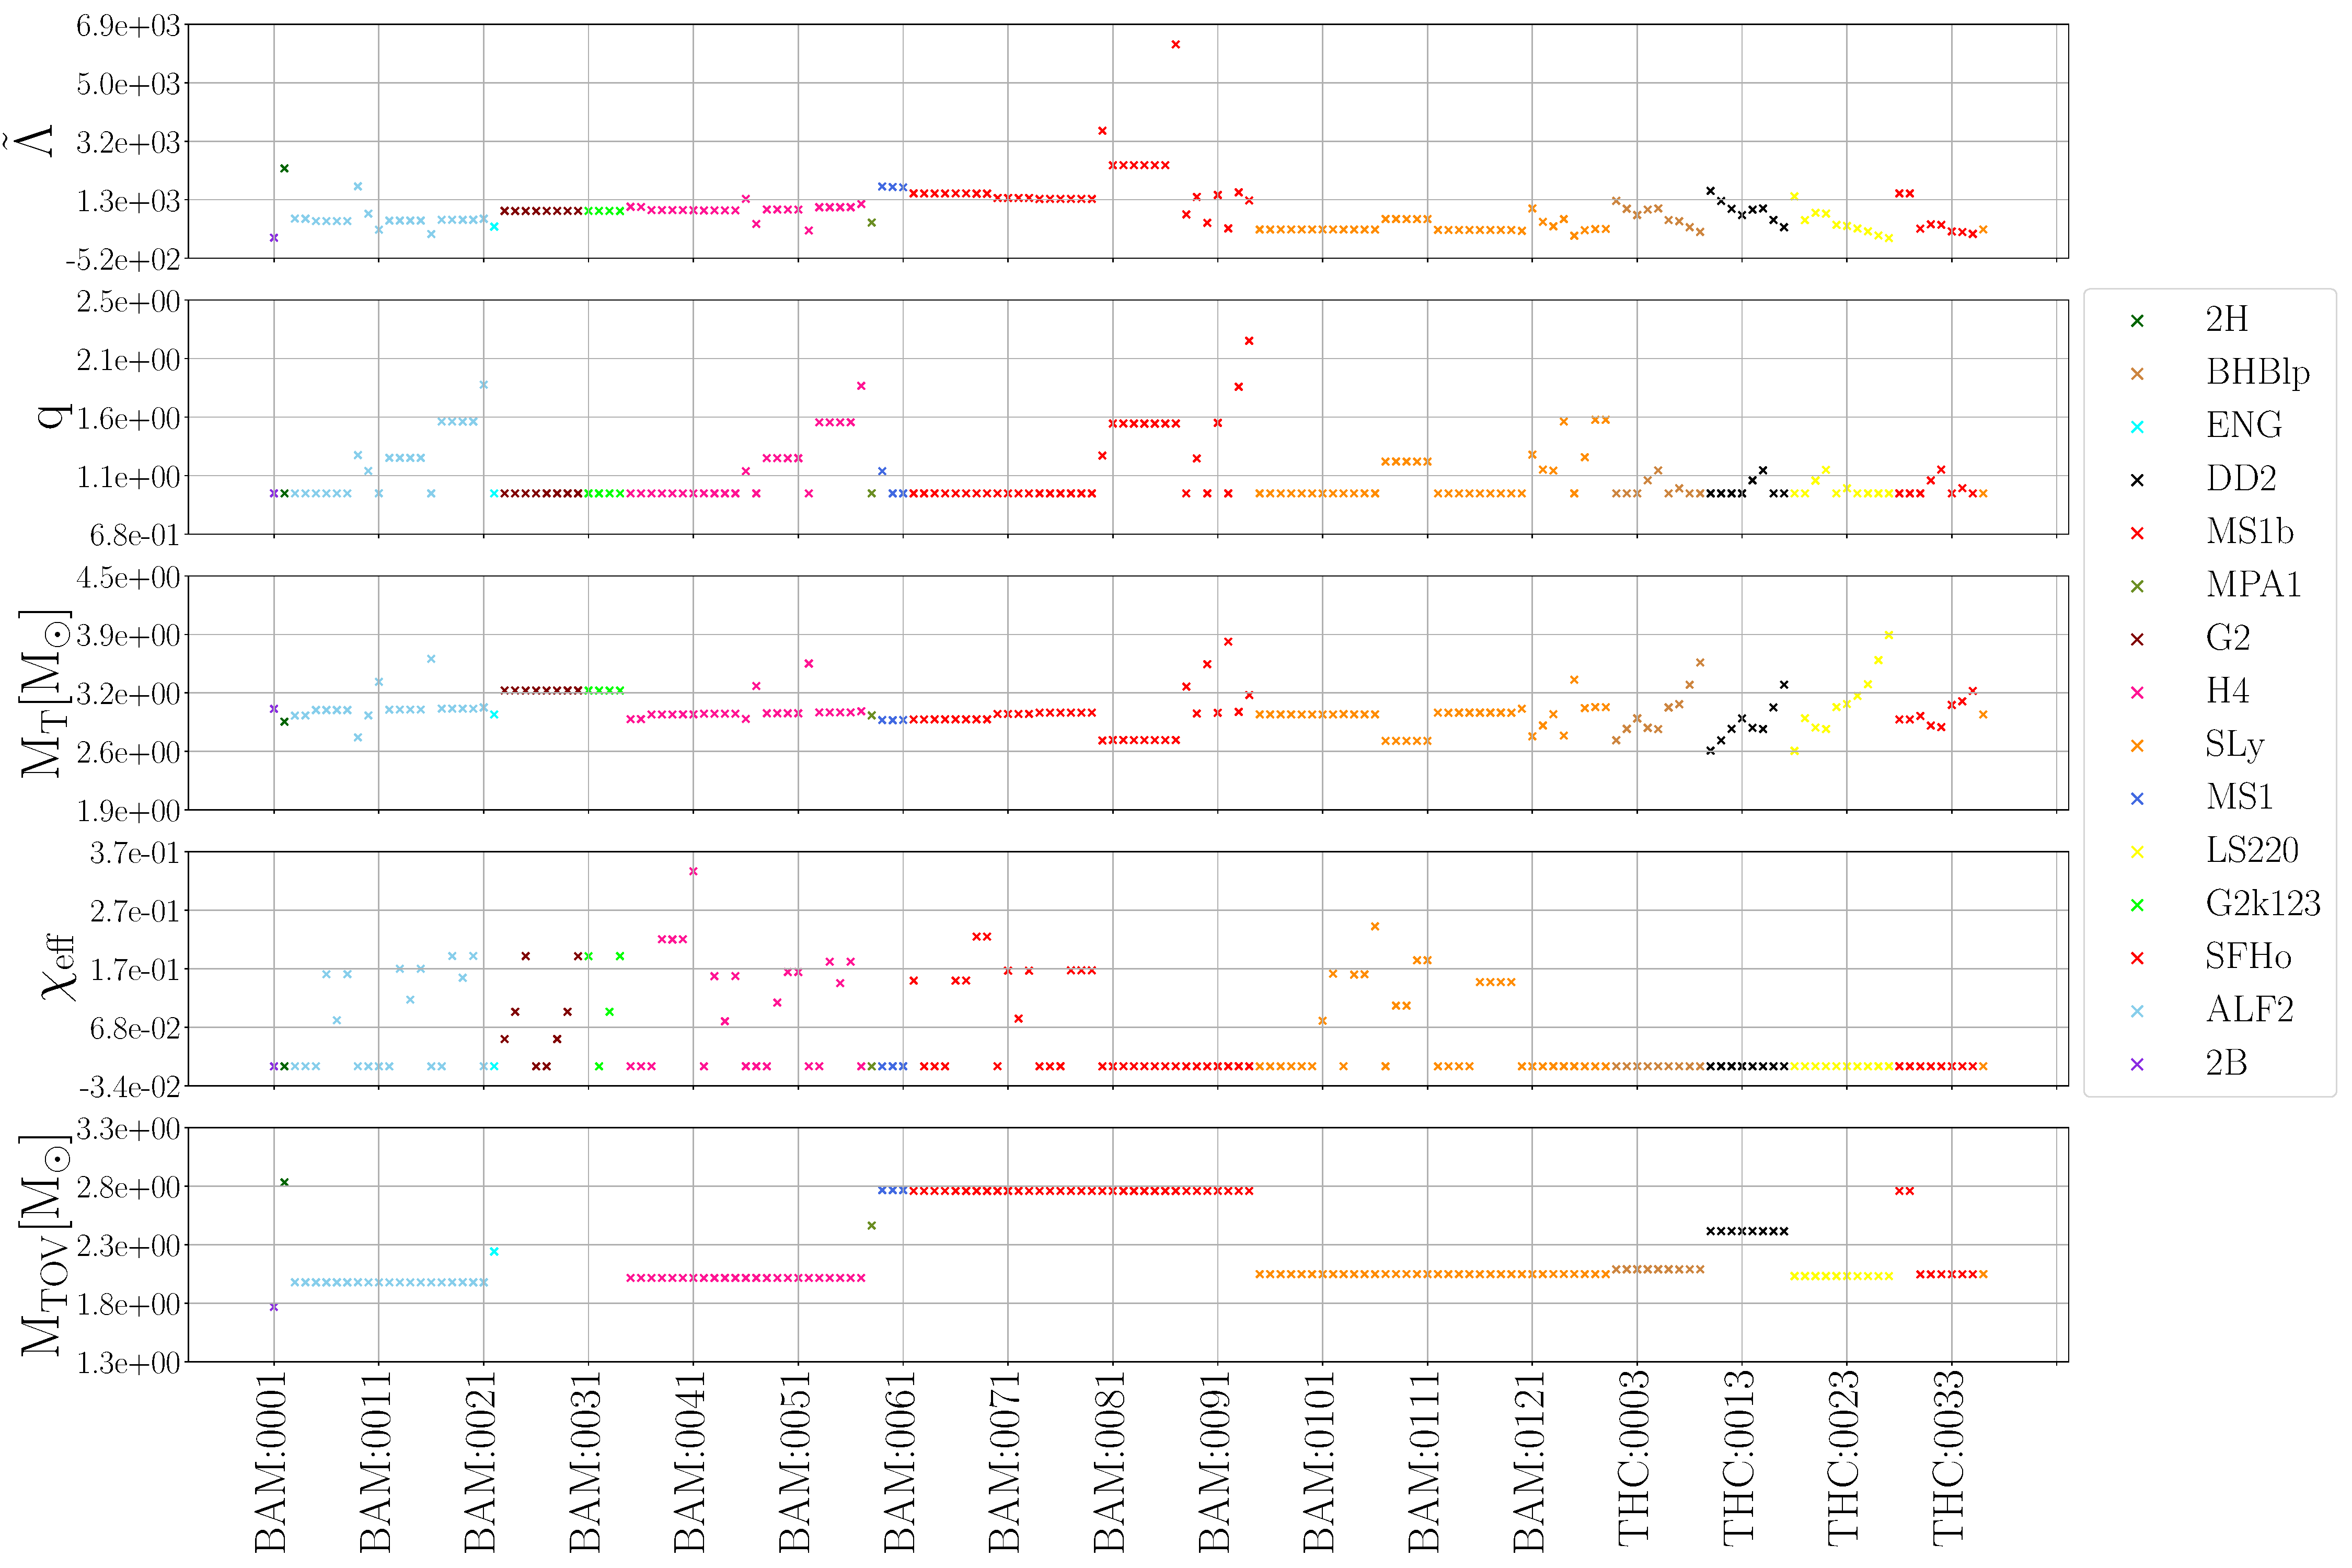
\includegraphics[width=\textwidth]{images/Data_analysis/results/CORE_cat.pdf} 
\captionsetup{width=0.8\textwidth}
\caption[CoRe BNS catalog metadata]{CoRe BNS catalog metadata. This type of layered plot helps represent simulation metadata according to the simulation IDs shown on the x-axis. The simulations in the CoRe catalog\cite{Dietrich:2018phi} provide information about the spins, masses, and tidal deformability.}
\end{center}
\label{corecat}
\end{figure}
\FloatBarrier

\newpage

In addition, the set of simulations computed by Kawamura et al. \cite{Kawamura:2016nmk}, De Petri et al. \cite{DePietri:2018tpx,DePietri:2015lya}, Feo et al. \cite{Feo:2016cbs}, Kastaun et al. \cite{Kastaun:2016elu}, Maione et al. \cite{Maione:2016zqz,Maione:2017aux} and Ciolfi et al. \cite{Ciolfi:2017uak} is also represented using a layered plot below.

\begin{figure}[hbt!]
\begin{center}
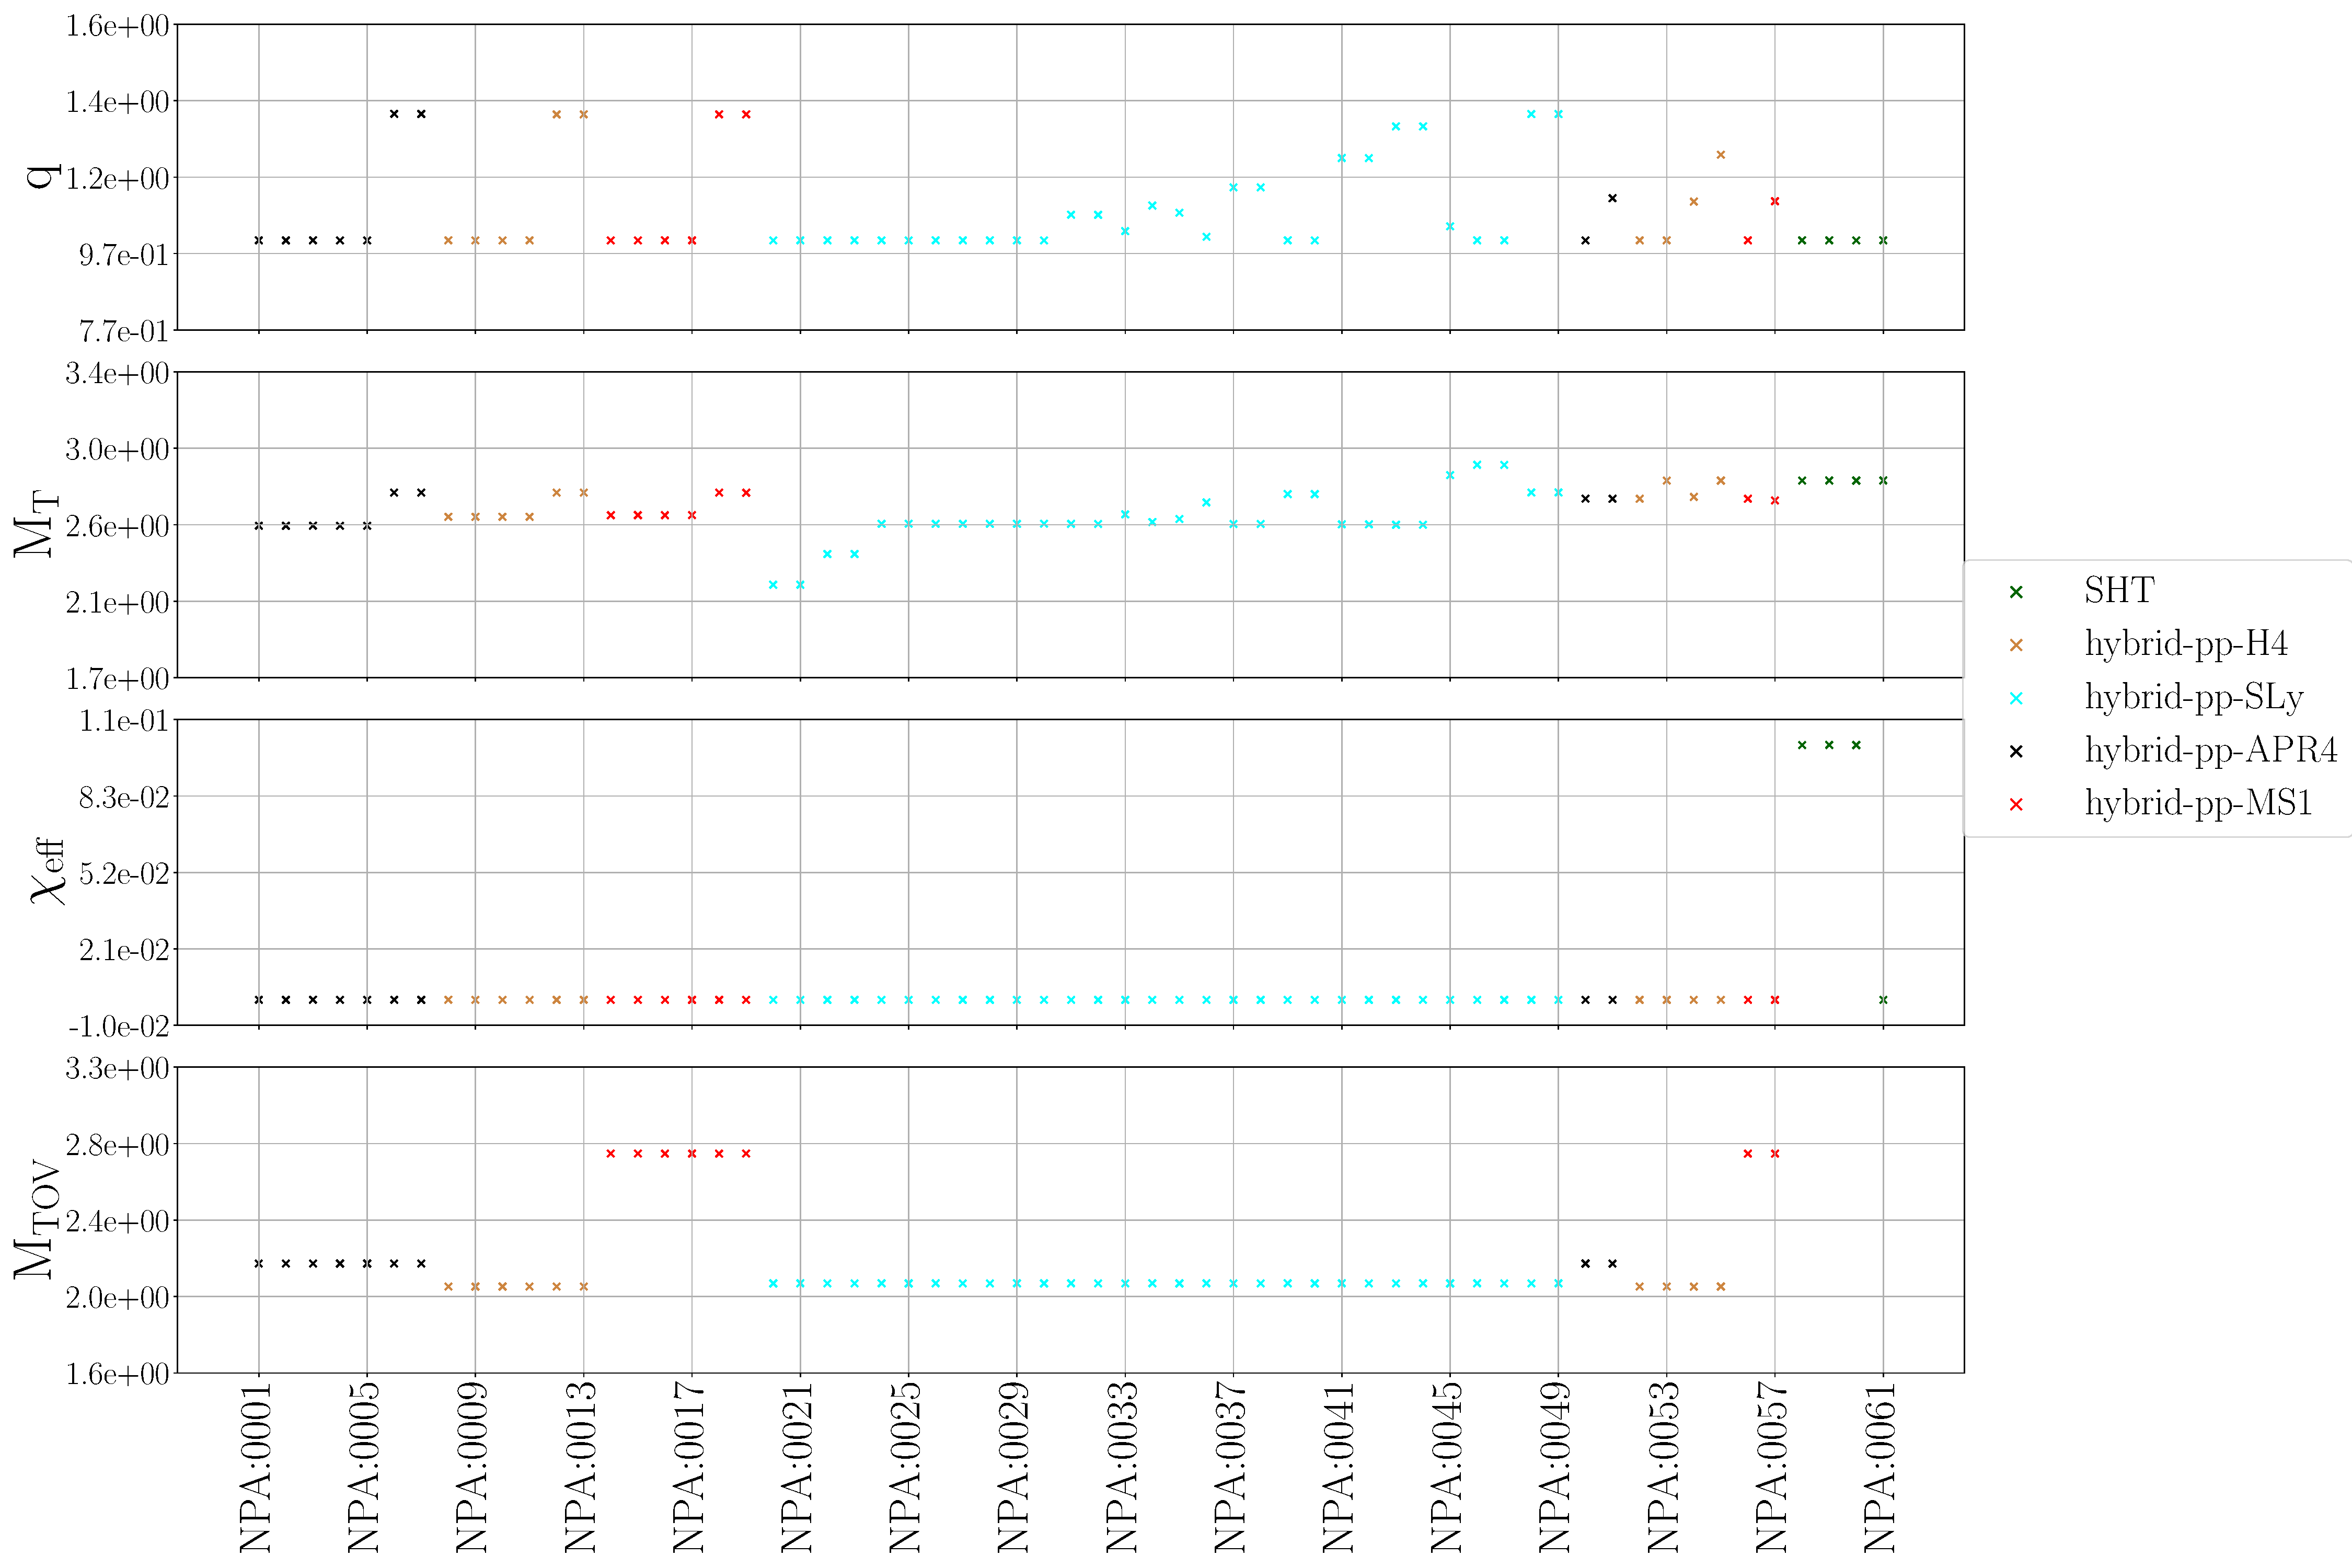
\includegraphics[width=\textwidth, angle=0]{images/Data_analysis/results/LAL_cat.pdf} 
\captionsetup{width=0.8\textwidth}
\caption[Metadata coming from other waveforms outside the CoRe catalog]{Metadata for waveforms. This type of layered plot helps represent simulation metadata according to the simulation IDs shown on the x-axis. Waveforms represented in this figure were computed by Kawamura et al. \cite{Kawamura:2016nmk}, De Petri et al. \cite{DePietri:2018tpx,DePietri:2015lya}, Feo et al. \cite{Feo:2016cbs}, Kastaun et al. \cite{Kastaun:2016elu}, Maione et al. \cite{Maione:2016zqz,Maione:2017aux} and Ciolfi et al. \cite{Ciolfi:2017uak}. Dots are colored according to the Equation of state(right).}
\end{center}
\label{lalcat}
\end{figure}

\FloatBarrier


